% axi-cylinder.tex

\newpage
\section{Viscous Flow Along a Cylinder}
\label{axi-cylinder-sec}
%
This case (\texttt{2D/axi-cylinder/} computes the flow for
a supersonic laminar boundary layer growing along a hollow cylinder.
It was used in the original report\cite{jacobs_91d} to verify the implementation of
the viscous and axisymmetric terms in the code.

\begin{figure}[htbp]
\begin{center}
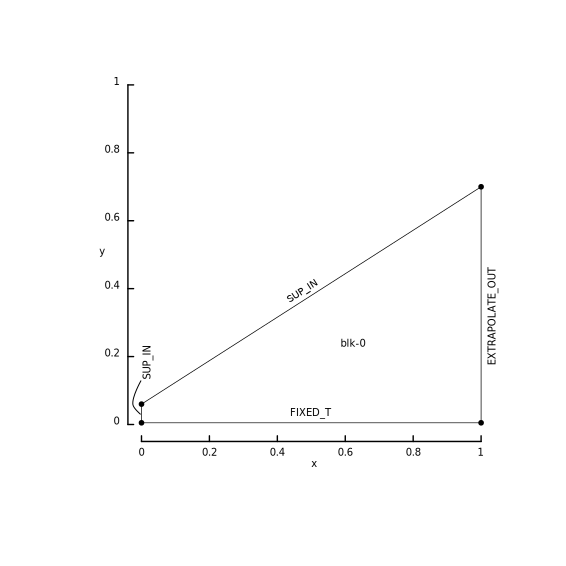
\includegraphics[width=0.7\textwidth,viewport=79 77 400 392,clip=true]{../2D/axi-cylinder/cyl50.pdf}
\end{center}
\caption{Flow domain for viscous flow along a cylinder.}
   \label{cyl50-layout-fig}
\end{figure}

\medskip
The flow geometry consists of a hollow cylinder, 1.0m long with
radius 0.005m, aligned with the $x$-axis.
The flow domain shown in Figure~\ref{cyl50-layout-fig} is defined
by a quadrilateral with corners (1.0,~0.005), (1.0,~0.7),
(0.0,~0.06), (0.0,~0.005).
This region is shaped to capture the weak leading-edge-interaction shock 
while concentrating cells near the cylinder surface for the early part of the boundary layer development.
The grid consists of $50 \times 50$ cells which are clustered toward
the leading edge of the cylinder and 
(even more strongly in the $y$-direction) toward the cylinder surface.

\medskip
The free stream is a uniform supersonic flow of air, modelled
as a perfect gas with conditions
$$
   \rho = 0.00404~ {\rm kg/m^3},~~
   u_x = 597.3~ {\rm m/s}, ~~
   u_y = 0, ~~
   e = C_v T = 1.592 \times 10^5 ~ {\rm J/kg},
$$
%
$$
   T = 222~ {\rm K}, ~~
   p = 257~ {\rm Pa}, ~~
   M = 2.
$$
This free stream condition is applied to the West and North
boundaries, the East boundary is a supersonic outflow boundary and
the South boundary (along the cylinder surface) is a no-slip
boundary with temperature fixed at $T = 222~\rm K$.
The Reynolds number at the end of the plate is $1.65 \times 10^5$.

\medskip
Initially, the flow throughout the block is set at the same conditions
as the free stream and the governing equations are integrated in time.
Figure~\ref{cyl50-flow-field-fig} shows the pressure and temperature fields
after a period of 8\,ms.
The weak leading-edge interaction shock is most clearly seen in the pressure field
and the boundary layer on the cylinder surface is evident in the temperature field.

\begin{figure}[htbp]
\mbox{
\includegraphics[width=0.5\textwidth]{../2D/axi-cylinder/cyl50-t8ms-p.png}
\includegraphics[width=0.5\textwidth]{../2D/axi-cylinder/cyl50-t8ms-T.png}
}
\caption{Pressure and temperature fields for viscous flow along a cylinder.}
   \label{cyl50-flow-field-fig}
\end{figure}

\medskip
Figure \ref{cyl50-profiles-fig} shows the $x$-velocity and temperature profiles
through the boundary layer at $x$=0.916\,m, 
48 cells from the leading edge of the cylinder.
The simulation data from \texttt{Eilmer3} are compared with data produced by David Pruett's
spectral boundary layer code.

\begin{figure}[htbp]
\mbox{
\includegraphics[width=0.5\textwidth]{../2D/axi-cylinder/cyl50_profile_ux.pdf}
\includegraphics[width=0.5\textwidth]{../2D/axi-cylinder/cyl50_profile_T.pdf}
}
\caption{Velocity and temperature profiles at $x = 0.916$\,m for viscous flow along a cylinder.}
   \label{cyl50-profiles-fig}
\end{figure}

\medskip
This case requires a fairly large computational effort of about 4 hours to reach
a simulation time of 8\,ms.


\newpage
\subsection{Input script (.py)}
\topbar
\lstinputlisting[language={}]{../2D/axi-cylinder/cyl50.py}
\bottombar


\subsection{Shell scripts}
\label{axi-cylinder-sh-files}
\topbar
\lstinputlisting[language={}]{../2D/axi-cylinder/cyl50_run.sh}
\bottombar

\noindent
\topbar
\lstinputlisting[language={}]{../2D/axi-cylinder/cyl50_plot.sh}
\bottombar


\subsection{Notes}
\begin{itemize}
\item None
\end{itemize}


